\section{Постоянный электрический ток}

\begin{ex}
Найти сопротивление цепи между точками $A$ и $B$. Сопротивление каждого резистора известно и равно $R$.
\begin{center}
\begin{tikzpicture}[european]
	\draw (-0.5,0) to [short, o-] (0,0) to [R=$R$] (2,0) to [R=$R$] (4,0) to [R=$R$] (6,0) to [short, -o] (6.5,0) 
	(0,0) to [short, *-] (0,1) -- (4,1) to [short, -*]  (4,0)
	(2,0) to [short, *-] (2,-1) -- (6,-1) to  [short, -*] (6,0)
	(-0.5,0.25) node[]{$A$}
	(6.5,0.25) node[]{$B$};
\end{tikzpicture}
\end{center}
\begin{figure}[H]
\centering
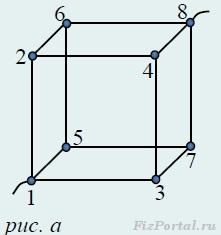
\includegraphics[scale=0.5]{1101DirectCurrentABCircuitCube.jpg}
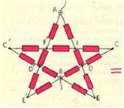
\includegraphics[scale=1]{1101DirectCurrentABCircuitStar.jpg}
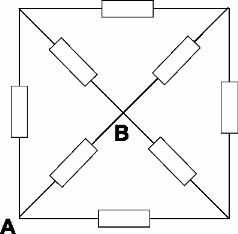
\includegraphics[scale=0.5]{1101DirectCurrentABCircuitSquare.jpg}
\end{figure}
\begin{ans}
$R/3$, $5R/6$, $6R/7$, $7R/15$
\end{ans}
\end{ex}

\begin{ex}
\hspace{0pt} \\
\begin{minipage}{.65\textwidth}
Сопротивления резисторов $R_1 = 1$ Ом, $R_2 = 2$ Ом, $R_3 = 3$ Ом, $R_4 =4$ Ом. 
Напряжение источника тока $U = 1$ В. Найдите ток, который течет через перемычку.
\end{minipage}
\begin{minipage}{.35\textwidth}
\centering
\begin{tikzpicture}[european, scale=0.9]
	\draw (1.5,0) to [short, o-] (0,0) -- (0,-2) to [R=$R_3$] (2,-2) to [R=$R_4$] (4,-2) -- (4,0)  to [short, -o] (2.5,0)
	(0,-1) to [R=$R_1$, *-] (2,-1) to [R=$R_2$] (4,-1) to [short, -*] (4,-1)
	(2,-1) to [short, *-*] (2,-2)
	(2,0) node[]{$U$};
\end{tikzpicture}
\end{minipage}
\begin{ans}
$I = 2/21$ А
\end{ans}
\end{ex}

\begin{ex}
\hspace{0pt} \\
\begin{minipage}{.65\textwidth}
Три одинаковых медных кольца радиуса $r$ соединены так, как показано на рисунке. 
Найдите сопротивление полученной таким образом фигуры, внешнее напряжение подано к точкам $A$ и $B$. 
Удельное сопротивление меди $\rho$, диаметр проволоки~$d$.
\end{minipage}
\begin{minipage}{.35\textwidth}
\centering
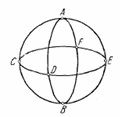
\includegraphics[width = 0.8 \textwidth]{1103DirectCurrentThreeRings.jpg}
\end{minipage}
\begin{ans}
$R = \rho r /16d^2$
\end{ans}
\end{ex}

\begin{ex}
Найдите эквивалентное сопротивление между точками $A$ и $B$ бесконечной цепочки, которая состоит из одинаковых резисторов сопротивлением $R$ каждый.
\begin{figure}[H]
\centering
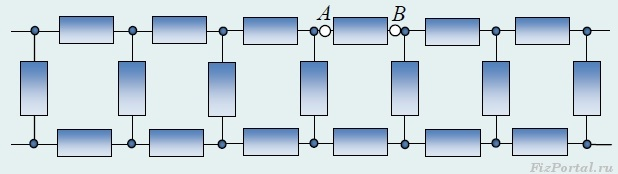
\includegraphics[scale=0.5]{1104DirectCurrentFourInfiniteCircuitAB.jpg}
\end{figure}
\begin{ans}
$(6-\sqrt{3})R/6$
\end{ans}
\end{ex}

\begin{ex}
\hspace{0pt} \\
\begin{minipage}{.65\textwidth}
Из бесконечной проводящей квадратной сетки, каждое звено которой имеет сопротивление $R$, удалили одно звено $AB$. Найдите сопротивление сетки между точками $A$ и $B$.
\end{minipage}
\begin{minipage}{.35\textwidth}
\centering
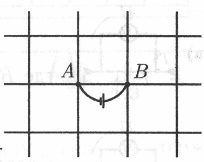
\includegraphics[width = 0.8 \textwidth]{1105DirectCurrentNet.jpg}
\end{minipage}
\begin{ans}
$R$
\end{ans}
\end{ex}

\begin{ex}
Имеется $n$ клемм, каждая из которых соединена со всеми остальными клеммами одинаковыми проводниками сопротивлением $R$. Найдите сопротивление между любыми двумя клеммами.
\begin{ans}
$R_1 = 2R/n$
\end{ans}
\end{ex}

\begin{ex}
Электрический чайник имеет две обмотки. При включении одной из них чайник вскипает через 10 мин, при включении другой -- через 15 мин. 
Через какое время чайник вскипит, если эти две обмотки включить вместе параллельно, последовательно?
\begin{ans}
$t_1 = 6$ мин, $t_2 = 25$ мин
\end{ans}
\end{ex}

\begin{ex}
\hspace{0pt} \\
\begin{minipage}{.65\textwidth}
На рисунке представлен график зависимости силы тока от напряжения на нелинейном резисторе. 
Определите силу тока в цепи при подключении этого резистора к источнику тока с напряжением 10 В и добавочным сопротивлением 100 Ом.
\end{minipage}
\begin{minipage}{.35\textwidth}
\centering
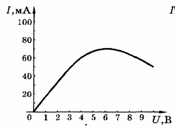
\includegraphics[width = 0.9 \textwidth]{1108DirectCurrentVDR.jpg}
\end{minipage}
\begin{ans}
$I = 0,06$ А
\end{ans}
\end{ex}

\begin{ex}
\hspace{0pt} \\
\begin{minipage}{.65\textwidth}
На рисунке приведен график зависимости напряжения на разрядном промежутке дугового разряда от тока. Дугу подключают  к источнику постоянного напряжения последовательно с резистором. 
При каком максимальном значении сопротивления резистора дуга может гореть при напряжении источника $U =85$~В?
\end{minipage}
\begin{minipage}{.35\textwidth}
\centering
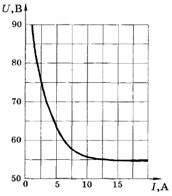
\includegraphics[width = 0.9 \textwidth]{1109DirectCurrentArcDischarge.jpg}
\end{minipage}
\begin{ans}
$R = 5$ Ом
\end{ans}
\end{ex}

\begin{ex}
\hspace{0pt} \\
\begin{minipage}{.65\textwidth}
Схема, изображенная на рисунке, состоит из двух одинаковых резисторов $R_2$ и $R_3$ сопротивлением $R$ каждый и двух одинаковых нелинейных резисторов $R_1$ и $R_4$, вольтамперная характеристика которых имеет вид $U = \alpha I^2$. При каком напряжении источника питания $U_0$ сила тока через гальванометр равна нулю?
\end{minipage}
\begin{minipage}{.35\textwidth}
\centering
\begin{tikzpicture}[european, scale=0.9]
	\draw (1.5,0) to [short, o-] (0,0) -- (0,-3) to [R, l=$R_3$] (2,-3) to [thR, l=$R_4$] (4,-3) -- (4,0)  to [short, -o] (2.5,0)
	(0,-1) to [thR, l=$R_1$, *-] (2,-1) to [R, l=$R_2$] (4,-1) to [short, -*] (4,-1)
	(2,-1) to [ammeter, *-*] (2,-3)
	(2,0) node[]{$U_0$};
\end{tikzpicture}
\end{minipage}
\begin{ans}
$U_0 = 2R^2/\alpha$
\end{ans}
\end{ex}

\begin{ex}
(2018) Проволочный предохранитель перегорает при напряжении 300 В. При каком напряжении будет перегорать предохранитель, если его длину увеличить в 3 раза, a диаметр -- в 2 раза?
\begin{ans}
636 В
\end{ans}
\end{ex}